\documentclass{standalone}
\usepackage{tikz}
\usetikzlibrary{patterns, positioning}
\usepackage[sfdefault]{ClearSans} %% option 'sfdefault' activates Clear Sans as the default text font
\usepackage[T1]{fontenc}

\begin{document}
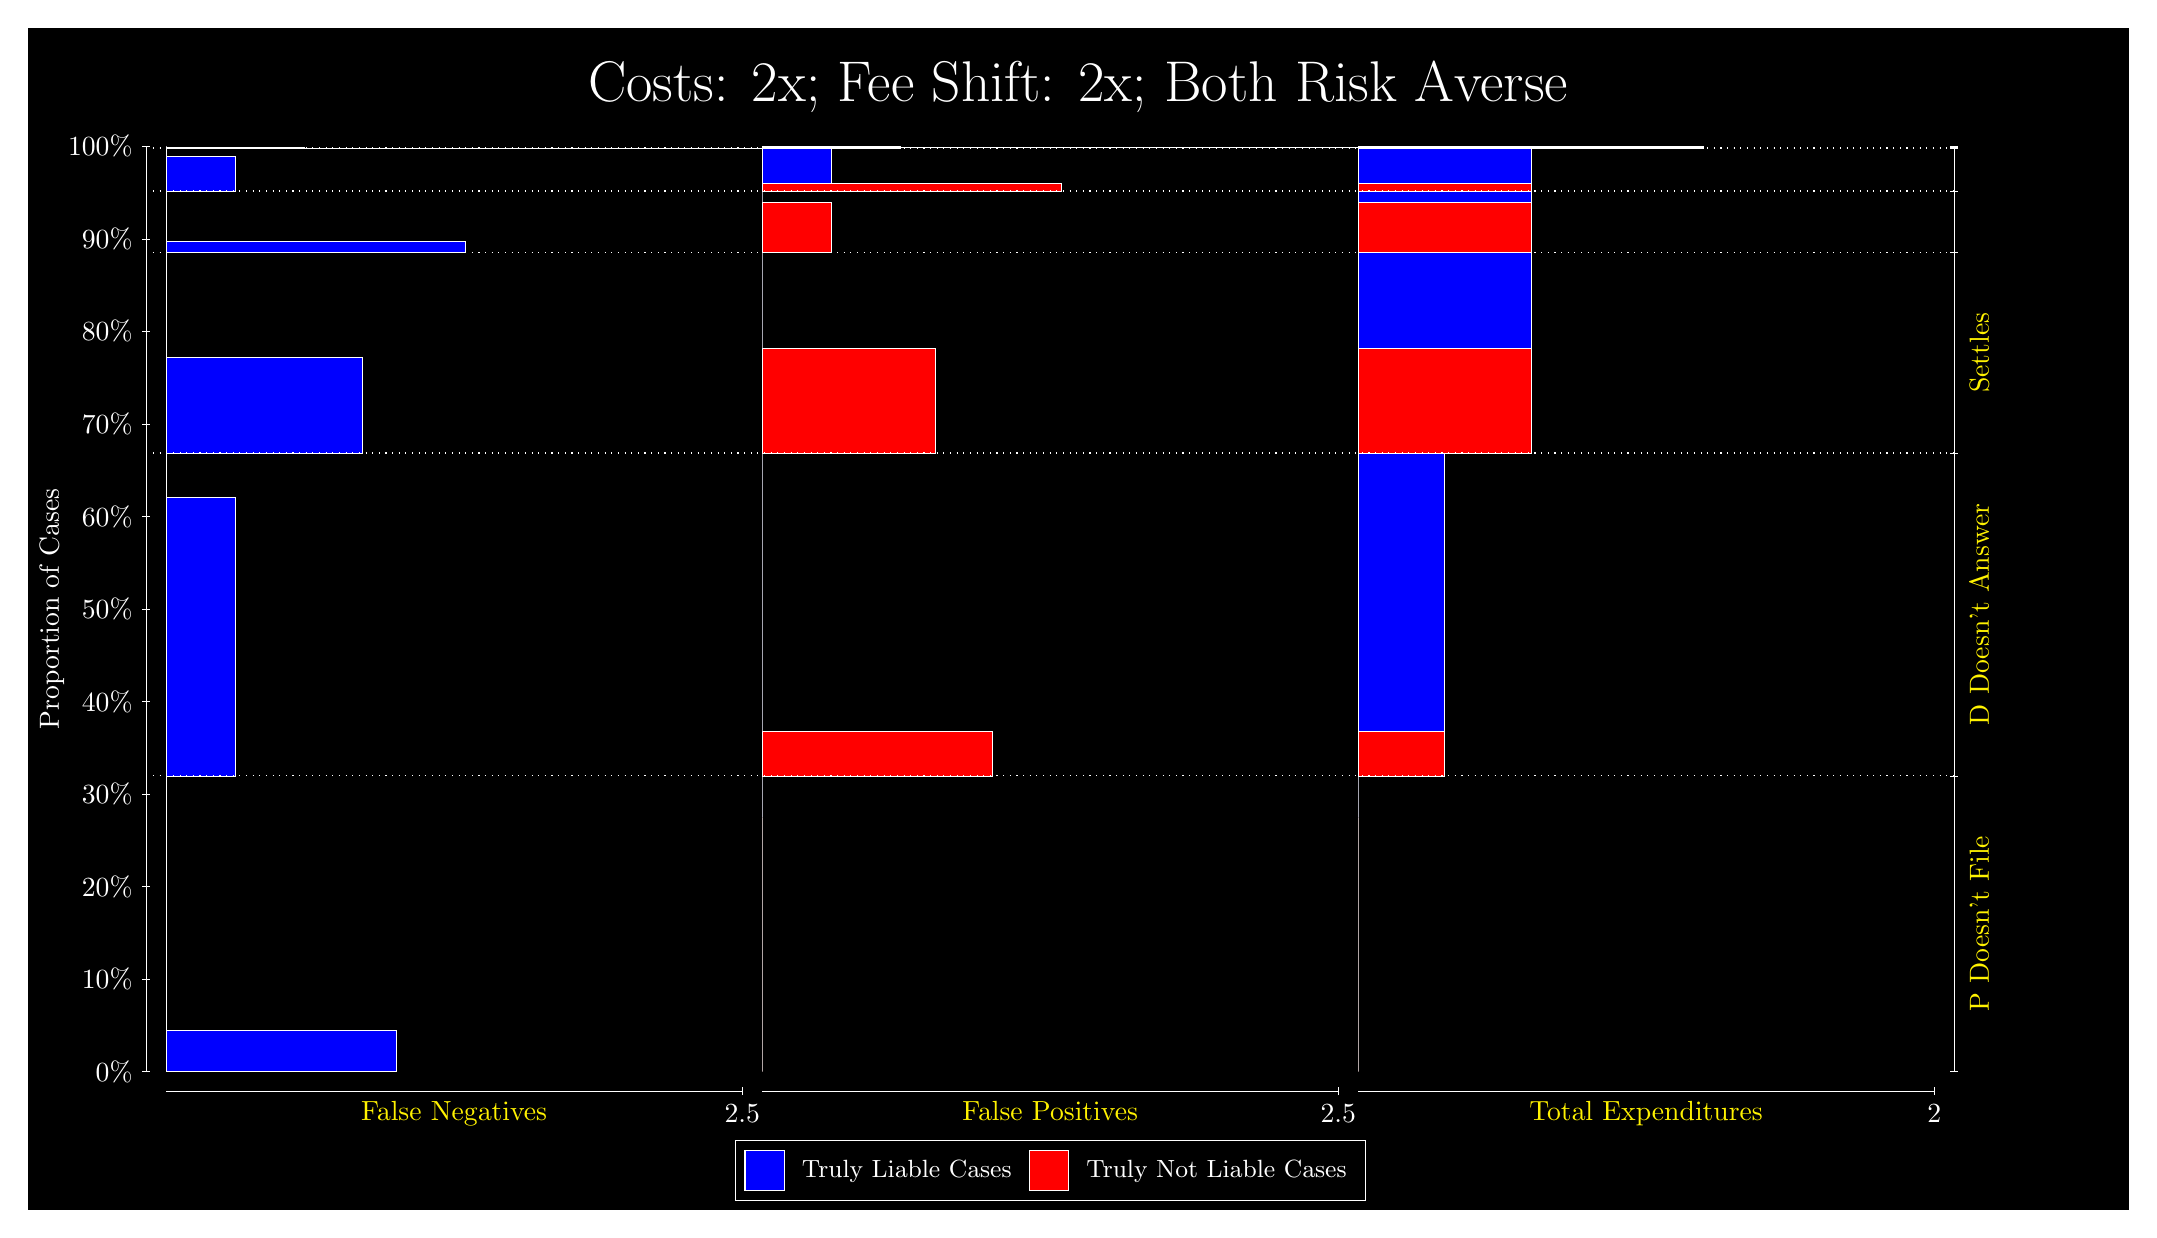
\begin{tikzpicture}
\draw[fill=black] (0,0) rectangle (26.667,15);
\draw[text=white] (0,13.5) rectangle (26.667,15) node[midway] {\huge Costs: 2x; Fee Shift: 2x; Both Risk Averse};
\draw[white, very thin] (1.5,1.75) -- (1.5,13.5);
\node[rotate=90, text=white, anchor=center] at (0.3, 7.625) {Proportion of Cases};
\draw[white, very thin] (1.45,1.75) -- (1.55,1.75);
\node[text=white, anchor=east] at (1.45, 1.75) {0\%};
\draw[white, very thin] (1.45,2.925) -- (1.55,2.925);
\node[text=white, anchor=east] at (1.45, 2.925) {10\%};
\draw[white, very thin] (1.45,4.1) -- (1.55,4.1);
\node[text=white, anchor=east] at (1.45, 4.1) {20\%};
\draw[white, very thin] (1.45,5.275) -- (1.55,5.275);
\node[text=white, anchor=east] at (1.45, 5.275) {30\%};
\draw[white, very thin] (1.45,6.45) -- (1.55,6.45);
\node[text=white, anchor=east] at (1.45, 6.45) {40\%};
\draw[white, very thin] (1.45,7.625) -- (1.55,7.625);
\node[text=white, anchor=east] at (1.45, 7.625) {50\%};
\draw[white, very thin] (1.45,8.8) -- (1.55,8.8);
\node[text=white, anchor=east] at (1.45, 8.8) {60\%};
\draw[white, very thin] (1.45,9.975) -- (1.55,9.975);
\node[text=white, anchor=east] at (1.45, 9.975) {70\%};
\draw[white, very thin] (1.45,11.15) -- (1.55,11.15);
\node[text=white, anchor=east] at (1.45, 11.15) {80\%};
\draw[white, very thin] (1.45,12.325) -- (1.55,12.325);
\node[text=white, anchor=east] at (1.45, 12.325) {90\%};
\draw[white, very thin] (1.45,13.5) -- (1.55,13.5);
\node[text=white, anchor=east] at (1.45, 13.5) {100\%};

\draw[white, very thin] (24.457,1.75) -- (24.457,13.5);
\draw[white, very thin] (24.407,1.75) -- (24.507,1.75);
\node[anchor=west] at (24.407, 1.75) {};
\draw[white, very thin] (24.407,5.5054) -- (24.507,5.5054);
\node[anchor=west] at (24.407, 5.5054) {};
\draw[white, very thin] (24.407,9.6057) -- (24.507,9.6057);
\node[anchor=west] at (24.407, 9.6057) {};
\draw[white, very thin] (24.407,12.152) -- (24.507,12.152);
\node[anchor=west] at (24.407, 12.152) {};
\draw[white, very thin] (24.407,12.933) -- (24.507,12.933);
\node[anchor=west] at (24.407, 12.933) {};
\draw[white, very thin] (24.407,13.474) -- (24.507,13.474);
\node[anchor=west] at (24.407, 13.474) {};
\draw[white, very thin] (24.407,13.487) -- (24.507,13.487);
\node[anchor=west] at (24.407, 13.487) {};
\draw[white, very thin] (24.407,13.5) -- (24.507,13.5);
\node[anchor=west] at (24.407, 13.5) {};

\draw[white, very thin, fill=blue] (1.75,1.75) rectangle (4.6775,2.277);
\draw[white, very thin, fill=red] (1.75,2.277) rectangle (1.75,5.5054);
\draw[white, very thin, fill=blue] (1.75,5.5054) rectangle (2.6283,9.0428);
\draw[white, very thin, fill=red] (1.75,9.0428) rectangle (1.75,9.6057);
\draw[white, very thin, fill=blue] (1.75,9.6057) rectangle (4.2384,10.823);
\draw[white, very thin, fill=red] (1.75,10.823) rectangle (1.75,12.152);
\draw[white, very thin, fill=blue] (1.75,12.152) rectangle (5.5558,12.293);
\draw[white, very thin, fill=red] (1.75,12.293) rectangle (1.75,12.933);
\draw[white, very thin, fill=blue] (1.75,12.933) rectangle (2.6283,13.373);
\draw[white, very thin, fill=red] (1.75,13.373) rectangle (1.75,13.474);
\draw[white, very thin, fill=blue] (1.75,13.474) rectangle (9.9471,13.475);
\draw[white, very thin, fill=blue] (1.75,13.475) rectangle (6.4341,13.479);
\draw[white, very thin, fill=red] (1.75,13.479) rectangle (1.75,13.487);
\draw[white, very thin, fill=blue] (1.75,13.487) rectangle (3.5065,13.493);
\draw[white, very thin, fill=red] (1.75,13.493) rectangle (1.75,13.498);
\draw[white, very thin, fill=blue] (1.75,13.498) rectangle (1.75,13.5);
\draw[white, very thin, fill=red] (9.3189,1.75) rectangle (9.3189,4.9783);
\draw[white, very thin, fill=blue] (9.3189,4.9783) rectangle (9.3189,5.5054);
\draw[white, very thin, fill=red] (9.3189,5.5054) rectangle (12.246,6.0683);
\draw[white, very thin, fill=blue] (9.3189,6.0683) rectangle (9.3189,9.6057);
\draw[white, very thin, fill=red] (9.3189,9.6057) rectangle (11.515,10.935);
\draw[white, very thin, fill=blue] (9.3189,10.935) rectangle (9.3189,12.152);
\draw[white, very thin, fill=red] (9.3189,12.152) rectangle (10.197,12.793);
\draw[white, very thin, fill=blue] (9.3189,12.793) rectangle (9.3189,12.933);
\draw[white, very thin, fill=red] (9.3189,12.933) rectangle (13.125,13.035);
\draw[white, very thin, fill=blue] (9.3189,13.035) rectangle (10.197,13.474);
\draw[white, very thin, fill=red] (9.3189,13.474) rectangle (11.075,13.48);
\draw[white, very thin, fill=red] (9.3189,13.48) rectangle (9.3189,13.482);
\draw[white, very thin, fill=blue] (9.3189,13.482) rectangle (9.3189,13.487);
\draw[white, very thin, fill=red] (9.3189,13.487) rectangle (17.516,13.487);
\draw[white, very thin, fill=blue] (9.3189,13.487) rectangle (14.588,13.49);
\draw[white, very thin, fill=red] (9.3189,13.49) rectangle (14.003,13.494);
\draw[white, very thin, fill=blue] (9.3189,13.494) rectangle (11.075,13.5);
\draw[white, very thin, fill=red] (16.888,1.75) rectangle (16.888,4.9783);
\draw[white, very thin, fill=blue] (16.888,4.9783) rectangle (16.888,5.5054);
\draw[white, very thin, fill=red] (16.888,5.5054) rectangle (17.986,6.0683);
\draw[white, very thin, fill=blue] (16.888,6.0683) rectangle (17.986,9.6057);
\draw[white, very thin, fill=red] (16.888,9.6057) rectangle (19.083,10.935);
\draw[white, very thin, fill=blue] (16.888,10.935) rectangle (19.083,12.152);
\draw[white, very thin, fill=red] (16.888,12.152) rectangle (19.083,12.793);
\draw[white, very thin, fill=blue] (16.888,12.793) rectangle (19.083,12.933);
\draw[white, very thin, fill=red] (16.888,12.933) rectangle (19.083,13.035);
\draw[white, very thin, fill=blue] (16.888,13.035) rectangle (19.083,13.474);
\draw[white, very thin, fill=red] (16.888,13.474) rectangle (21.279,13.48);
\draw[white, very thin, fill=blue] (16.888,13.48) rectangle (21.279,13.484);
\draw[white, very thin, fill=red] (16.888,13.484) rectangle (21.279,13.486);
\draw[white, very thin, fill=blue] (16.888,13.486) rectangle (21.279,13.487);
\draw[white, very thin, fill=red] (16.888,13.487) rectangle (21.279,13.491);
\draw[white, very thin, fill=blue] (16.888,13.491) rectangle (21.279,13.497);
\draw[white, very thin, fill=red] (16.888,13.497) rectangle (21.279,13.498);
\draw[white, very thin, fill=blue] (16.888,13.498) rectangle (21.279,13.5);
\draw[white, dotted] (1.5,5.5054) -- (24.457,5.5054);
\draw[white, dotted] (1.5,9.6057) -- (24.457,9.6057);
\draw[white, dotted] (1.5,12.152) -- (24.457,12.152);
\draw[white, dotted] (1.5,12.933) -- (24.457,12.933);
\draw[white, dotted] (1.5,13.474) -- (24.457,13.474);
\draw[white, dotted] (1.5,13.487) -- (24.457,13.487);
\draw[white, very thin] (1.75,1.5) -- (9.0689,1.5);
\node[text=yellow, anchor=north] at (5.4094, 1.5) {False Negatives};
\draw[white, very thin] (9.0689,1.45) -- (9.0689,1.55);
\node[text=white, anchor=north] at (9.0689, 1.45) {2.5};

\draw[white, very thin] (9.3189,1.5) -- (16.638,1.5);
\node[text=yellow, anchor=north] at (12.978, 1.5) {False Positives};
\draw[white, very thin] (16.638,1.45) -- (16.638,1.55);
\node[text=white, anchor=north] at (16.638, 1.45) {2.5};

\draw[white, very thin] (16.888,1.5) -- (24.207,1.5);
\node[text=yellow, anchor=north] at (20.547, 1.5) {Total Expenditures};
\draw[white, very thin] (24.207,1.45) -- (24.207,1.55);
\node[text=white, anchor=north] at (24.207, 1.45) {2};

\node[text=yellow, centered, rotate=90] at (24.777, 3.6277) {P Doesn't File};
\node[text=yellow, centered, rotate=90] at (24.777, 7.5555) {D Doesn't Answer};
\node[text=yellow, centered, rotate=90] at (24.777, 10.879) {Settles};





\draw (12.978300999999998,1.5) node[draw=none] (baseCoordinate) {};
\begin{scope}[align=center]
        \matrix[scale=0.5, draw=white, below=0.5cm of baseCoordinate, nodes={draw}, column sep=0.1cm]{
            \node[rectangle, draw, minimum width=0.5cm, minimum height=0.5cm, fill=blue] {}; &
            \node[draw=none, font=\small, text=white] (B) {Truly Liable Cases}; &
            \node[rectangle, draw, minimum width=0.5cm, minimum height=0.5cm, fill=red] {}; &
            \node[draw=none, font=\small, text=white] (B) {Truly Not Liable Cases}; \\
            };
\end{scope}

\end{tikzpicture}
\end{document}